% =============================================================================
% FRESCO manuscript -- Springer Nature research-article structure.
%
% Template note: this source uses the standard article class so that it compiles
% anywhere (tectonic/pdflatex). For submission, switch to the official Springer
% Nature template (sn-jnl.cls, version 3.1, Dec 2024, from the publisher's author
% pages or Overleaf gallery):
%   \documentclass[pdflatex,sn-mathphys-num]{sn-jnl}
% and map: \title -> \title[short]{...}; authors -> \author*[1]{...}\affil*[1]{...};
% abstract -> \abstract{...}; keywords -> \keywords{...}; Declarations -> \bmhead{...}.
% The section structure below already follows the template.
%
% STATUS: working manuscript. Every empirical result is SYNTHETIC (simulator with
% known ground truth). Real-agent results are explicit [TO RUN] placeholders.
% Not submission-ready until Section 9.9 is filled from executed experiments and
% the author/declaration placeholders are completed.
% =============================================================================
\documentclass[11pt]{article}
\usepackage[a4paper,margin=2.4cm]{geometry}
\usepackage[T1]{fontenc}
\usepackage{lmodern}
\usepackage{amsmath,amssymb,amsthm}
\usepackage{booktabs,tabularx,array}
\usepackage{graphicx}
\usepackage[numbers,sort&compress]{natbib}
\usepackage{algorithm}
\usepackage{algpseudocode}
\usepackage{xcolor}
\usepackage{tikz}
\usetikzlibrary{arrows.meta,positioning,fit,backgrounds}
\usepackage[font=small,labelfont=bf]{caption}
\usepackage[colorlinks=true,linkcolor=blue!50!black,citecolor=blue!50!black,urlcolor=blue!50!black]{hyperref}
\graphicspath{{../figures/}}

\newtheorem{theorem}{Theorem}
\newtheorem{proposition}[theorem]{Proposition}
\newtheorem{corollary}[theorem]{Corollary}
\newtheorem{assumption}{Assumption}
\theoremstyle{definition}
\newtheorem{definition}{Definition}
\theoremstyle{remark}
\newtheorem{remark}{Remark}
\newcommand{\todo}[1]{\textcolor{red!70!black}{[#1]}}
\newcommand{\E}{\mathbb{E}}
\newcommand{\Prob}{\Pr}
\newcommand{\bhat}{\hat b}
\renewcommand{\algorithmicrequire}{\textbf{Input:}}
\renewcommand{\algorithmicensure}{\textbf{Output:}}

\title{FRESCO: Fault-Tolerant, Anytime-Valid Distributed Estimation of\\ Counterfactual Security Margins for LLM Agents}
\author{\todo{AUTHOR NAMES AND AFFILIATIONS --- INSERT AND VERIFY BEFORE SUBMISSION}}
\date{Working manuscript, 18 October 2026 --- simulation results only; real-agent results pending}

\begin{document}
\maketitle

\begin{abstract}
\noindent\textbf{Purpose.} Counterfactual security margins summarise how much adversarial intervention an LLM agent tolerates before it commits an unauthorized action. Estimating them requires many stochastic, adaptively chosen agent episodes, so evaluations are run on distributed harnesses with retries, at-least-once queues and elastic workers. We study whether such execution preserves the statistical guarantees of the estimate.
\textbf{Methods.} We formulate margin confirmation as anytime-valid sequential testing with betting e-processes and per-candidate error spending (LEXIS), and design FRESCO, a ledger-based distributed protocol whose six rules (seed-committed slots, prefix-predictable bets, exactly-once in-order commit, direction-aware crash imputation, a global leased error budget, and verifiable confirmation) make validity independent of scheduling. We prove validity under adaptive generation, arbitrary stopping, message loss, duplication, reordering, crashes and partitions, and show by construction that removing any single rule admits executions whose false-confirmation probability approaches one. We evaluate an implementation in a deterministic fault-injection simulator with known ground truth.
\textbf{Results.} In simulation, FRESCO kept the false-confirmation probability at or below 0.018 (nominal 0.05) in every configuration, including combined faults; removing deduplication, the fresh-retry ban or in-order commit raised it to 0.083--0.133. FRESCO reached the true margin 25.4$\times$ faster with 32 workers (efficiency 0.79) at about 3.5 messages per oracle call. Two preregistered hypotheses failed: cooperation gave no detectable speed-up over independent runs with a split error budget, and LEXIS was less sample-efficient than a repaired fixed-design procedure; a screening hybrid closed most of that gap (reaching the margin in 0.756 versus 0.808 of runs) but not all of it. The fixed-design procedure as originally specified in MARGIN-Bench exceeded its nominal error (0.257).
\textbf{Conclusion.} Distributed execution semantics are part of the statistics of security evaluation. FRESCO provides fault-tolerant validity at negligible coordination cost; it does not provide a cooperative or sample-efficiency advantage. Real-agent validation is specified but not yet executed.
\end{abstract}

\noindent\textbf{Keywords:} LLM agents; adversarial robustness; security evaluation; anytime-valid inference; e-values; distributed systems; fault tolerance; reproducibility

% -----------------------------------------------------------------------------
\section{Introduction}\label{sec:intro}

Tool-using language-model agents read untrusted content, call services and delegate to other agents, and their security failures are \emph{actions}: an unauthorized ledger update, a forwarded secret, a privilege change~\cite{greshake2023,debenedetti2024agentdojo,zhan2024injecagent}. MARGIN-Bench~\cite{marginbench2026} proposes to report not only whether an agent can be compromised but the smallest identified intervention cost at which a violation becomes reproducible---a counterfactual safety margin per attack surface. Its estimand is
\begin{equation}
R_{s,\alpha}(M,E)=\inf\{\,c_s(\delta)\;:\;\delta\in A_s(E),\ p_M(E,\delta)\ge\alpha\,\},\label{eq:margin}
\end{equation}
where $p_M(E,\delta)$ is the probability that intervention $\delta$ on surface $s$ yields a committed violation, and $\alpha$ a reproducibility threshold.

Estimating~\eqref{eq:margin} is computationally heavy. Each candidate intervention must be executed repeatedly because agents are stochastic; candidates are generated adaptively; and a benchmark multiplies this over hundreds of scenario bundles, four attack surfaces, several budgets and models, yielding on the order of $10^7$--$10^8$ agent episodes. Such workloads run on distributed harnesses, and the default semantics of those harnesses---at-least-once delivery, retry-on-failure with fresh randomness, results consumed as they arrive, worker-local configuration---are designed for throughput, not for statistical validity.

This paper's central observation is that \emph{these execution semantics are part of the statistics}. A sequential test that consumes a duplicated result, a retried episode whose first attempt crashed because it was long, or results ordered by latency is no longer testing the hypothesis it reports. We show that each such default can drive the probability of falsely confirming a vulnerability far above its nominal level, and we design a protocol under which it cannot.

\paragraph{Contributions.}
\begin{enumerate}
\item[C1] \textbf{Schedule-oblivious validity.} We formulate margin confirmation as anytime-valid testing with betting e-processes and registration-time error spending (LEXIS) and prove that the reported margin is a $(1-\varepsilon)$ upper confidence bound on~\eqref{eq:margin} for any generator, allocation, stopping rule and execution order, provided evidence is consumed by slot index (Theorem~\ref{thm:lexis}). Validity is thereby decoupled from scheduling: any scheduler is safe.
\item[C2] \textbf{FRESCO protocol.} A ledger-based protocol with six rules that realises the conditions of C1 under message loss, duplication, reordering, crash-stop failures and partitions (Theorem~\ref{thm:fresco}), with a necessity result: removing any single rule admits executions whose false-confirmation probability approaches one (Theorem~\ref{thm:necessity}).
\item[C3] \textbf{Two-sided reporting.} Anytime-valid cost-level certificates that bound the attack generator's violating mass at searched budgets without claiming a lower bound on the margin itself (Propositions~\ref{prop:zf}--\ref{prop:cs}).
\item[C4] \textbf{Implementation and evaluation.} A tested implementation, a deterministic fault-injection simulator, and a preregistered synthetic evaluation including two negative results (no cooperative speed-up; lower sample efficiency than a repaired fixed design), and a preregistered screening + e-process hybrid that closes most, but not all, of the efficiency gap.
\item[C5] \textbf{Audit of the baseline estimator.} The confirmation procedure specified in MARGIN-Bench lacks a correction across budget levels and exceeds its nominal error by a factor of five; we give and evaluate a repair.
\end{enumerate}

\paragraph{Non-claims.} We do not claim a certified lower bound on the margin, a speed-up from cooperation, better sample efficiency than well-designed fixed procedures, validity when episodes share hidden state, or any finding about real agents: all empirical results are synthetic, with real-agent experiments specified in Section~\ref{sec:realprotocol} and not yet executed.

% -----------------------------------------------------------------------------
\section{Research problem}\label{sec:problem}

Let a scenario $E$, surface $s$ and defender $M$ be fixed. An adaptive generator proposes candidates $\delta_1,\delta_2,\dots$ with integer costs $c(\delta_j)\in\{1,\dots,K\}$. Executing candidate $j$ with randomness key $u$ yields $Y(\delta_j,u)\in\{0,1\}$, the committed-violation label of a permission-grounded oracle. The evaluator wants to report $\bhat$, the smallest cost at which some candidate is \emph{confirmed} to satisfy $p(\delta)\ge\alpha$, such that
\begin{equation}
\Prob(R_{s,\alpha} > \bhat)\le\varepsilon,\label{eq:G1}
\end{equation}
while executing episodes on $W$ unreliable workers. The research question, posed as a falsifiable hypothesis rather than assumed, is: \emph{Can distributed workers discover and confirm low-cost violations faster than a single process while preserving~\eqref{eq:G1} under realistic faults, and does cooperation among them yield an advantage beyond parallelism?}

% -----------------------------------------------------------------------------
\section{Related work and novelty analysis}\label{sec:related}

\paragraph{Anytime-valid inference.} Test supermartingales, Ville's inequality and e-values provide inference valid under optional stopping~\cite{ramdas2023savi,vovk2021,grunwald2024safe}; betting confidence sequences~\cite{waudbysmith2024,howard2021} and always-valid A/B testing~\cite{johari2022} are mature, as are e-value multiple testing and online variants~\cite{wang2022ebh,xu2024online,foster2008}. Group-sequential designs handle delayed responses~\cite{hampson2013}. These methods assume a well-defined observation sequence; they do not address how a fault-prone distributed executor produces that sequence. Our contribution is not a new test but the identification of executor semantics that preserve or destroy the supermartingale property, with proofs and counterexamples.

\paragraph{Threshold and infinitely-armed bandits.} Good-arm identification~\cite{kano2019}, thresholding bandits~\cite{locatelli2016} and infinitely-armed pure exploration~\cite{aziz2018,chaudhuri2017} study finding arms above a threshold with bounded error; distributed exploration~\cite{hillel2013} and asynchronous successive halving~\cite{li2020asha} parallelise search. None targets the lexicographic \emph{cheapest-level} objective with per-level non-discovery certificates, and parallel systems optimise throughput rather than error control under faulty delivery. Our matching lower bound uses the change-of-measure argument of~\cite{kaufmann2016}.

\paragraph{Statistical assurance in testing.} Residual-risk estimation in fuzzing~\cite{bohme2018stads,bohme2021residual}, statistical model checking~\cite{younes2006,legay2010} and scenario optimisation~\cite{campi2008} bound what was not found; recent LLM-evaluation work stresses error bars~\cite{miller2024errorbars} and evidential limits of red teaming~\cite{kaur2026ceiling}. Our certificates are cost-indexed and anytime-valid but, as our experiments show, coarse at realistic budgets. Parallel fuzzing schedulers~\cite{dynamiq2025} remove redundancy for deterministic oracles; for stochastic confirmation, redundancy is a correctness issue.

\paragraph{Distributed systems.} We reuse leases~\cite{gray1989leases}, escrow~\cite{oneil1986escrow}, monotone state and coordination-freedom~\cite{shapiro2011crdt,hellerstein2020calm}, causal ordering and snapshots~\cite{lamport1978,chandy1985}, and list-scheduling bounds~\cite{graham1969}. The closest systems analogue is differential-privacy budget scheduling~\cite{luo2021privatekube}, which treats a non-replenishable statistical budget as a cluster resource; FRESCO's budget is a testing error budget spent at registration, validated by Ville and a union bound, and enforced alongside result deduplication and ordering, which DP budgeting does not need.

\paragraph{LLM agent security.} Benchmarks cover indirect injection, tool use, long-horizon and multi-agent attacks~\cite{debenedetti2024agentdojo,zhan2024injecagent,jiang2026agentlab,tamas2025,darkside2025,mazeika2024harmbench}; counterfactual and causal analyses separate permission from apparent risk~\cite{yang2026agentboundary,mothukuri2026causaltrace}; defences enforce capabilities and provenance~\cite{debenedetti2025camel,south2025delegation}; best-of-$N$ sampling shows that attack success grows with repeated stochastic trials~\cite{hughes2025bon}, which is exactly why confirmation must be statistical. Authorization consistency across agents~\cite{pang2019zanzibar,birgisson2014macaroons,lilienthal2025toctou} is related but orthogonal: we evaluate agents, not authorization infrastructure.

\begin{table}[t]\centering\small
\caption{Novelty positioning: what is reused and what is new.}\label{tab:novelty}
\begin{tabularx}{\linewidth}{>{\raggedright}p{3.0cm}>{\raggedright}X>{\raggedright\arraybackslash}X}
\toprule
Component & Established & New here \\\midrule
Per-candidate e-process & betting e-processes, Ville~\cite{waudbysmith2024,ramdas2023savi} & estimand is a lexicographic minimum over adaptively generated candidates; bets restricted to the committed prefix \\
Error spending & $\alpha$-investing, weighted Bonferroni~\cite{foster2008,genovese2006} & spending at registration from ledger leases with a polynomial schedule that never exhausts \\
Seed-committed in-order slots & deterministic replay; in-order commit & proved to make validity independent of execution order and latency (Thm.~\ref{thm:lexis}(iii)) \\
Crash imputation & worst-case imputation & direction-aware rule conservative for both confirmation and certification \\
Leased global budget & leases, escrow, DP budgets~\cite{gray1989leases,oneil1986escrow,luo2021privatekube} & testing-error budget with incarnation fencing; necessity shown by counterexample \\
Necessity results & --- & each executor default (duplicates, fresh retry, arrival order, local budget) breaks validity, some with error $\to1$ \\
\bottomrule\end{tabularx}
\end{table}

% -----------------------------------------------------------------------------
\section{Research questions and hypotheses}\label{sec:rq}
\begin{itemize}
\item \textbf{RQ1 (validity).} Does FRESCO keep false confirmation $\le\varepsilon$ under faults, and do executor defaults break it? (H-valid-sim, H-rules, H-alg1)
\item \textbf{RQ2 (scalability).} How does time-to-margin scale with workers, and what does coordination cost? (H-speed, H-overhead, H-recover)
\item \textbf{RQ3 (cooperation).} Does a shared ledger beat independent runs and a centralized scheduler? (H-coop)
\item \textbf{RQ4 (efficiency and certificates).} Is LEXIS at least as sample-efficient as a fixed design, and are certificates calibrated? (H-vs-Alg1, H-cert)
\end{itemize}
Decision criteria were fixed before the full runs (after a 3-seed pilot used only for sizing) and are listed with verdicts in Table~\ref{tab:verdicts}.

% -----------------------------------------------------------------------------
\section{Framework and model}\label{sec:model}

\paragraph{Nodes and trust.} A logically single, linearizable \emph{ledger} holds all authoritative state; \emph{workers} (honest, crash-stop, elastic) run generators and request slots; \emph{executors} run one sandboxed agent episode per slot from an immutable snapshot and evaluate the oracle. The generator is untrusted with respect to the statistics: it may exploit any leakage, sees only committed outcomes, and never sees a slot's key before the slot is registered and leased. The network may delay, reorder, duplicate and drop messages and partition. Byzantine workers are out of scope: workers belong to the evaluator.

\begin{assumption}[Fresh-key conditional Bernoulli]\label{as:a1}
Slot $(j,k)$ uses a key $u_{j,k}$; keys are i.i.d.\ and independent of the generator's randomness, and $Y_{j,k}=Y(\delta_j,u_{j,k})$. Executions share no hidden state.
\end{assumption}
\begin{assumption}[Registration before revelation]\label{as:a2} No party learns $u_{j,\cdot}$ before candidate $j$ is registered with its error weight fixed.\end{assumption}
\begin{assumption}[Crash independence]\label{as:a4} Whether slot $(j,k)$ crashes may depend on its own key and trajectory and on infrastructure noise independent of all other keys. (Not needed in replay mode.)\end{assumption}
\begin{assumption}[Oracle correctness]\label{as:a5} $Y$ is the true committed-violation label; with false-positive rate $\omega$ all guarantees hold for $p+\omega(1-p)$.\end{assumption}

Under drift, all results hold for the null ``$p_{j,k}\le\alpha$ at every slot''; a confirmation then means the violation probability exceeded $\alpha$ at some time during the run.

\paragraph{Targets.} (G1) $\Prob(R>\bhat)\le\varepsilon$, implied by the no-false-witness property $\Prob(\exists j\text{ confirmed}: p(\delta_j)\le\alpha)\le\varepsilon$. (G2) For audit distributions $D_k$ and $\mu_k=D_k\{p\ge\alpha_c\}$, certificates $\bar\eta_k$ with $\Prob(\exists k:\mu_k>\bar\eta_k)\le\varepsilon'$. No statement $R>b$ is ever produced.

% -----------------------------------------------------------------------------
\section{LEXIS: anytime-valid margin confirmation}\label{sec:lexis}

For candidate $j$ with null $H_j:p(\delta_j)\le\alpha$ define
\begin{equation}
E_{j,n}=\prod_{i=1}^{n}\bigl(1+\lambda_{j,i}(\tilde Y_{j,i}-\alpha)\bigr),\qquad \lambda_{j,i}=f_j(\mathcal R_j,\tilde Y_{j,1},\dots,\tilde Y_{j,i-1})\in[0,1/\alpha),\label{eq:eproc}
\end{equation}
where $\mathcal R_j$ is the registration information (including the weight $a_j$) and $\tilde Y$ the recorded outcome. Candidate $j$ is confirmed once $\sup_n E_{j,n}\ge 1/a_j$, and $\bhat=\min\{c(\delta_j): j\text{ confirmed}\}$. Weights satisfy $\sum_j a_j\le\varepsilon$ almost surely; by default lease $n$ receives $\varepsilon/(n(n+1))$, split evenly across $R$ registrations, which never exhausts.

\begin{theorem}[Schedule-oblivious validity]\label{thm:lexis}
Under Assumptions~\ref{as:a1}--\ref{as:a4}, if $\tilde Y\le Y$ pointwise, bets depend only on registration information and the committed prefix, and the committed stream of each candidate is a prefix of its slot-indexed sequence, then for every generator, allocation and continuation policy, stopping rule and execution order, $\Prob(\exists j: H_j\text{ true},\ j\text{ confirmed})\le\varepsilon$, hence $\Prob(R>\bhat)\le\varepsilon$.
\end{theorem}
\begin{proof}
Index candidates by registration and extend each slot sequence to infinity conceptually. Let $E^*_{j,n}$ be~\eqref{eq:eproc} on the full sequence and $\mathcal G_{j,n}=\sigma(\mathcal R_j,\tilde Y_{j,1..n},\text{crash noise of slots }1..n)$. (i) By Assumptions~\ref{as:a1}, \ref{as:a2} and \ref{as:a4}, $u_{j,n+1}$ is independent of $\mathcal G_{j,n}$, so $\E[\tilde Y_{j,n+1}\mid\mathcal G_{j,n}]\le\E[Y_{j,n+1}\mid\mathcal G_{j,n}]=p(\delta_j)\le\alpha$ under $H_j$; with $\lambda\ge0$ predictable and $1-\lambda\alpha>0$, $E^*_j$ is a non-negative supermartingale with $E^*_{j,0}=1$. (ii) Ville's inequality conditional on $\mathcal R_j$ gives $\Prob(\sup_n E^*_{j,n}\ge1/a_j\mid\mathcal R_j)\le a_j$ on $H_j$. (iii) Whatever the schedule, the committed stream is a prefix of the full sequence, so confirmation implies $\sup_nE^*_{j,n}\ge1/a_j$; abandonment, pruning, out-of-order execution and even clairvoyant stopping only shorten the prefix. (iv) Summing, the probability that some true null is confirmed is at most $\E\sum_ja_j\le\varepsilon$. If no null is confirmed, every confirmed $\delta$ has $p>\alpha$, so $R\le\bhat$.
\end{proof}

\begin{proposition}[Anytime zero-failure certificate]\label{prop:zf}
For i.i.d.\ Bernoulli($q$) draws and any random time $N$, $\Prob\bigl(S_N=0\text{ and }q>1-\beta^{1/N}\bigr)\le\beta$.
\end{proposition}
\begin{proof}
With $n_0=\lceil\log\beta/\log(1-q)\rceil$ the event requires the first $n_0$ draws to be zero, which has probability $(1-q)^{n_0}\le\beta$.
\end{proof}

\begin{proposition}[Certificate from a betting upper confidence sequence]\label{prop:cs}
Test $H_g:q\ge g$ on a grid with $\prod(1+\lambda_i(g-Z_i))$, $\lambda_i$ predictable, and let $U_n$ be the smallest grid value above which all grid values are rejected. Then $\Prob(\exists n:q>U_n)\le\beta$. For audits $Z=\mathbf 1\{\ge t\text{ of }r\text{ runs violate}\}$ (crash $\Rightarrow Z=1$), every draw with $p\ge\alpha_c$ has $\Prob(Z=1)\ge h=\Prob(\mathrm{Bin}(r,\alpha_c)\ge t)$, so $\mu_k\le U_k/h=:\bar\eta_k$.
\end{proposition}
\begin{proof}
If $q>U_n$ the largest grid value $g\le q$ is rejected although $H_g$ holds; its e-process is a non-negative supermartingale, so Ville bounds this single event by $\beta$. Monotonicity of the binomial tail in $p$ gives the mass bound.
\end{proof}

\begin{proposition}[Confirmation cost]\label{prop:cost}
With a fixed bet $\lambda$ and drift $g(\lambda,p)>0$, $\E_p[\tau]\le(\log(1/a)+\log(1+\lambda(1-\alpha)))/g(\lambda,p)$, and the Kelly bet for $p_1$ attains $g=\mathrm{KL}(p_1\|\alpha)$. Any level-$a$ test that stops almost surely under $p$ has $\E_p[\tau]\ge\log(1/(2.4a))/\mathrm{KL}(p\|\alpha)$.
\end{proposition}
\begin{proof}
Wald's identity with bounded overshoot gives the upper bound; the lower bound is the change-of-measure argument of~\cite{kaufmann2016} applied to $\tau\wedge n$.
\end{proof}

Per-level search with candidates drawn i.i.d.\ and violating mass $\pi_k(\Delta)$ costs $O\bigl(K(\log\frac1\varepsilon+\log J)/(\pi_k\,\mathrm{KL}(\alpha{+}\Delta\|\alpha))\bigr)$ slots under uniform level weights, which are minimax among fixed weightings (worst case $T/\min_kw_k\ge KT$). Finally, the aggregate discovered-compromise curve $\hat F(b)=\frac1N\sum_i\mathbf 1\{\bhat_i\le b\}$ satisfies $\hat F(b)-F(b)\le\frac1N\sum_i\mathbf 1\{\bhat_i<R_i\}$ uniformly in $b$, so it is a conservative lower estimate of the vulnerable fraction up to $\varepsilon$ in expectation.

% -----------------------------------------------------------------------------
\section{FRESCO: protocol and architecture}\label{sec:fresco}

\begin{figure}[t]\centering
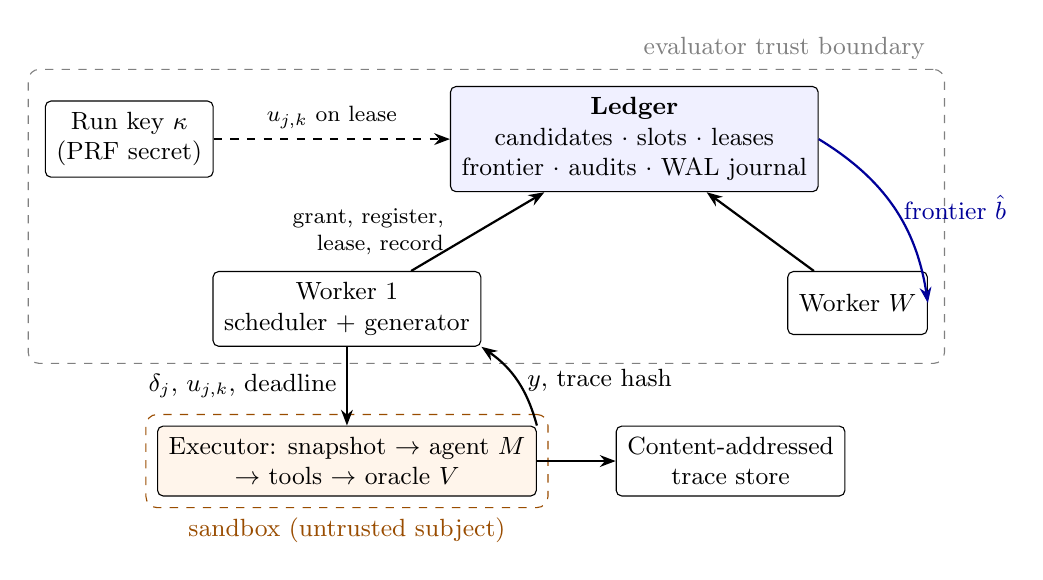
\begin{tikzpicture}[node distance=6mm and 10mm, every node/.style={font=\small},
  box/.style={draw, rounded corners=2pt, align=center, minimum height=8mm, inner sep=4pt},
  arr/.style={-{Stealth[length=2mm]}, thick}]
\node[box, fill=blue!6] (L) {\textbf{Ledger}\\ candidates $\cdot$ slots $\cdot$ leases\\ frontier $\cdot$ audits $\cdot$ WAL journal};
\node[box, left=30mm of L] (K) {Run key $\kappa$\\ (PRF secret)};
\node[box, below left=10mm and -4mm of L] (W1) {Worker 1\\ scheduler + generator};
\node[box, below right=10mm and -4mm of L] (W2) {Worker $W$};
\node[box, below=10mm of W1, fill=orange!8] (X) {Executor: snapshot $\to$ agent $M$\\ $\to$ tools $\to$ oracle $V$};
\node[box, right=10mm of X] (T) {Content-addressed\\ trace store};
\draw[arr, dashed] (K) -- node[above, font=\footnotesize]{$u_{j,k}$ on lease} (L);
\draw[arr] (W1) -- node[left=3mm, align=right, font=\footnotesize]{grant, register,\\ lease, record} (L);
\draw[arr] (W2) -- (L);
\draw[arr, blue!60!black] (L.east) to[bend left=25] node[right]{frontier $\bhat$} (W2.east);
\draw[arr] (W1) -- node[left]{$\delta_j$, $u_{j,k}$, deadline} (X);
\draw[arr] (X.north east) to[bend right=20] node[right]{$y$, trace hash} (W1.south east);
\draw[arr] (X) -- (T);
\begin{scope}[on background layer]
\node[draw=gray, dashed, rounded corners, fit=(L)(K)(W1)(W2), inner sep=6pt, label={[gray]above right:evaluator trust boundary}] {};
\node[draw=orange!60!black, dashed, rounded corners, fit=(X), inner sep=4pt, label={[orange!60!black]below:sandbox (untrusted subject)}] {};
\end{scope}
\end{tikzpicture}
\caption{FRESCO architecture. All safety properties route through the ledger; the frontier broadcast and worker state are soft caches that affect only efficiency.}\label{fig:arch}
\end{figure}

\paragraph{Rules.} \textbf{R1} slot keys $u_{j,k}=\mathrm{PRF}_\kappa(\text{run},j,k)$ revealed only on lease; \textbf{R2} bets see only the committed prefix; \textbf{R3} each slot has at most one terminal value (first write wins, fenced by a lease token) and the e-process consumes only the contiguous terminal prefix; \textbf{R4} a crashed slot is recorded as $Y=0$ for confirmation and $Z=1$ for audits and is never re-run with a fresh key (re-running with the \emph{same} key is allowed in replay mode); \textbf{R5} every weight is spent from a ledger lease bound to a worker incarnation and fenced on close; \textbf{R6} only the ledger confirms, by recomputing the e-process from stored slots.

\paragraph{State machine.} The ledger state is (candidates, slots, leases, frontier, audits). Transitions are guarded commands applied atomically and journaled before execution: \textsc{Grant}, \textsc{Register}, \textsc{Lease}, \textsc{Record}, \textsc{Expire}, \textsc{Advance}, \textsc{Prune}/\textsc{Abandon}, \textsc{Close}, \textsc{Audit}. Requests carry (sender, request id) and responses are cached, so retransmissions are idempotent; slot results are additionally fenced by token. Invariants I1--I7 (budget conservation, per-lease spending, write-once slots, monotone commit pointer, deterministic e-process, confirmation soundness, monotone frontier) are checked after every transition in property-based tests.

\begin{algorithm}[t]
\caption{FRESCO worker loop (any scheduling policy is valid by Theorem~\ref{thm:lexis})}\label{alg:worker}
\begin{algorithmic}[1]
\Loop
\If{no open lease} \State request \textsc{Grant} \EndIf
\State $\bhat_{\text{view}}\gets$ latest frontier (possibly stale)
\State $a\gets$ \Call{Schedule}{$\bhat_{\text{view}}$, local state}
\If{$a=\textsc{Audit}(k)$} \State lease audit $(k,i)$ with seed; draw $\delta\sim D_k(\text{seed})$; run $r$ episodes; \textsc{RecordAudit}
\ElsIf{$a=\textsc{New}(k)$} \State $\delta\gets G_k.\textsc{Propose}()$; \textsc{Register}(lease, $\delta$) \Comment{$a_j$ fixed here}
\ElsIf{$a=\textsc{Continue}(j,m)$}
  \For{each $(k,u,\text{tok})\in$ \textsc{Lease}$(j,m)$}
    \State $y\gets$ \textsc{Execute}$(\delta_j,u,\text{deadline})$; \textbf{if} no crash \textbf{then} \textsc{Record}$(j,k,y,\text{tok})$
  \EndFor
\EndIf
\EndLoop
\end{algorithmic}
\end{algorithm}

\begin{theorem}[Validity under asynchrony and faults]\label{thm:fresco}
Under Assumptions~\ref{as:a1}--\ref{as:a5} and rules R1--R6, G1 and G2 hold for every number of workers, membership history and interleaving, under message delay, reordering, duplication and loss, crash-stop failures of workers and executors, and network partitions.
\end{theorem}
\begin{proof}[Proof sketch]
Each hypothesis of Theorem~\ref{thm:lexis} is supplied by a rule: I3--I4 (R3) make the committed stream a prefix of one sequence, and duplicates and late messages fail the token guard; R4 gives $\tilde Y\le Y$ (a crash between execution and recording leaves the slot leased until expiry turns it into a recorded 0); R2 with R6 makes bets predictable; R1 gives Assumptions~\ref{as:a1}--\ref{as:a2}; I1--I2 with R5 give $\sum_ja_j\le\varepsilon$, since registrations under closed leases are rejected by the ledger. Partitions only delay transitions; the only timing-dependent transition (expiry) can only make recorded values more conservative. G2 follows from R4 and audit prefix commit with Propositions~\ref{prop:zf}--\ref{prop:cs}. In replay mode a re-run reproduces $Y(\delta_j,u_{j,k})$ exactly, so Assumption~\ref{as:a4} is not needed.
\end{proof}

\begin{theorem}[Necessity]\label{thm:necessity}
For each of R2, R3 (deduplication or ordering), R4 and R5 there is an execution satisfying all other rules with false-confirmation probability exceeding $\varepsilon$; for R3-ordering, R4 and R5 it tends to one.
\end{theorem}
\begin{proof}
Take $p=\alpha$. \emph{No dedup:} applying every result twice yields $(E^*)^2$; since $E^*$ is a martingale tending to zero, optional stopping gives error in $[\sqrt\varepsilon/(1+\lambda(1-\alpha)),\sqrt\varepsilon]$. \emph{Fresh retry:} if benign episodes crash with probability $c_0$ and violating ones with $c_1<c_0$, the recorded stream is Bernoulli$(p(1-c_1)/(p(1-c_1)+(1-p)(1-c_0)))>\alpha$ and any consistent test rejects almost surely. \emph{Arrival order:} with $m$ slots in flight and violations returning first, as $m\to\infty$ the consumed stream is $S\sim\mathrm{Bin}(N,\alpha)$ ones followed by zeros, which crosses any threshold for large $N$. \emph{Local budget:} $W$ workers each spending $\varepsilon$ give family-wise error $1-(1-\varepsilon_0)^W\to1$. \emph{Non-predictable bets:} betting with knowledge of the current outcome never loses wealth.
\end{proof}

\paragraph{Efficiency properties.} Because $\bhat$ is a monotone min-register computed by the ledger, frontier staleness $\Delta$ costs at most $KW\theta\Delta$ wasted slots ($\theta$ slots per worker per unit time) and never correctness; $m$ slots in flight per candidate waste at most $m-1$ per decision; and greedy scheduling gives $T_W\le Q_W\bar t/W+D\,T_{\max}$ with $D$ the generator's sequential depth~\cite{graham1969}. Coordination is one ledger write per slot plus one per registration; at agent-episode durations (5--60\,s) and $W=32$ this is under ten writes per second.

\paragraph{Component justification.} A single logical ledger (PostgreSQL in production; schema in the artifact) is required because every safety property needs one serialisation point. Message brokers, caches and custom consensus are deliberately absent: a broker adds an at-least-once hop that must then be deduplicated, a cache reintroduces stale reads that R6 avoids, and the ledger's database replication suffices for availability, which safety never depends on. General-purpose task frameworks may place executors but their automatic retries must be disabled, since they implement the fresh-retry pattern of Theorem~\ref{thm:necessity}.

% -----------------------------------------------------------------------------
\section{Experimental methodology}\label{sec:method}

\paragraph{Why simulation.} Coverage claims require ground truth (which candidates are null, the true margin $k^*$, the true masses $\mu_k$), which real agents never provide. We therefore evaluate the implemented protocol---ledger, message layer, workers---in a deterministic discrete-event simulator with Bernoulli oracles of known $p$, injected network faults (loss, duplication, reordering, partitions), worker and executor crashes, ledger crash with journal recovery, and outcome-correlated latency (lognormal, mean 20\,s benign / 30\,s violating). Same configuration and seed reproduce the same event trace.

\paragraph{Workloads.} S1-moderate: violating fractions $(0,0,0.05,0.10)$ at levels 1--4 with $p=0.6$; S2-sparse: $(0,0,0.01,0.05)$; weak scaling: $0.16/W$ at level 3; boundary null: every candidate at $p=\alpha=0.2$; certificate scenario: rare violators ($\mu=0.003,0.01$, $p=0.3$). $\alpha=0.2$, $\varepsilon=\varepsilon'=0.05$, four executors per worker, horizon $H=150{,}000$\,s.

\paragraph{Baselines.} B0a: MARGIN-Bench Algorithm~1 as specified (per-budget top-$T$ confirmation, Wilson bound at $\varepsilon/T$); B0b: repaired (Clopper--Pearson at $\varepsilon/(KT)$); B1: $W$ independent single-worker deployments with $\varepsilon/W$ each; B2: FRESCO with one rule removed; B3: one centralized scheduler driving all $4W$ executors. All methods use the same total concurrency.

\paragraph{Statistics.} Seeds are the unit of analysis. Time-to-margin is censored at $H$; we report restricted mean survival time (RMST) with percentile-bootstrap CIs, Kaplan--Meier curves~\cite{kaplan1958}, two-sided Mann--Whitney tests with Holm correction, rank-biserial correlations, and Wilson intervals for proportions. Validity is judged by the Wilson lower bound against $\varepsilon$. With 100 seeds per cell the study detects RMST ratios below about 0.65 with roughly 80\% power.

% -----------------------------------------------------------------------------
\section{Results}\label{sec:results}
All results in this section are synthetic.

\subsection{Validity (RQ1)}
Every ledger-based method stayed valid at every $W$ (Table~\ref{tab:validity}, Fig.~\ref{fig:validity}). Algorithm~1 as specified exceeded its nominal level five-fold: it tests $K=4$ budget levels in sequence, each at $\varepsilon/T$, without correcting across levels, and its Wilson bound is anti-conservative at $n=30$. The exact repair is valid and, as shown below, no less efficient. Rule ablations through the full system (400 seeds each) reproduced Theorem~\ref{thm:necessity}: removing deduplication, the fresh-retry ban or in-order commit gave 0.133 [0.103, 0.169], 0.102 [0.076, 0.136] and 0.083 [0.059, 0.114], against 0.003--0.018 for FRESCO under the same triggers and 0.003 [0.000, 0.014] under all faults combined. Removing the global budget at $W=8$ gave 0.065 [0.045, 0.094]; its inflation is not established at this configuration.

\begin{table}[t]\centering\small
\caption{False-confirmation probability on the boundary null (every confirmation is false; nominal $\varepsilon=0.05$; 95\% Wilson intervals).}\label{tab:validity}
\begin{tabular}{lrl}
\toprule
Method & False/runs & $\Prob$(false confirmation) \\\midrule
FRESCO, $W=1$ / 8 / 32 & 5, 2, 1 / 400 & 0.013, 0.005, 0.003 (all upper limits $\le0.029$) \\
Independent $\varepsilon/W$, $W=8$ / 32 & 2, 0 / 400 & 0.005, 0.000 \\
Centralized scheduler, $W=8$ / 32 & 9, 6 / 400 & 0.022 [0.012, 0.042], 0.015 [0.007, 0.032] \\
Algorithm 1 as specified (Wilson, $\varepsilon/T$) & 513/2000 & \textbf{0.257 [0.238, 0.276]} \\
Algorithm 1 repaired (Clopper--Pearson, $\varepsilon/KT$) & 69/2000 & 0.035 [0.027, 0.043] \\
LEXIS (1,160 / 30,000-slot budget) & 37, 21 / 2000 & 0.018 [0.013, 0.025], 0.011 [0.007, 0.016] \\
\bottomrule\end{tabular}
\end{table}

\begin{figure}[t]\centering
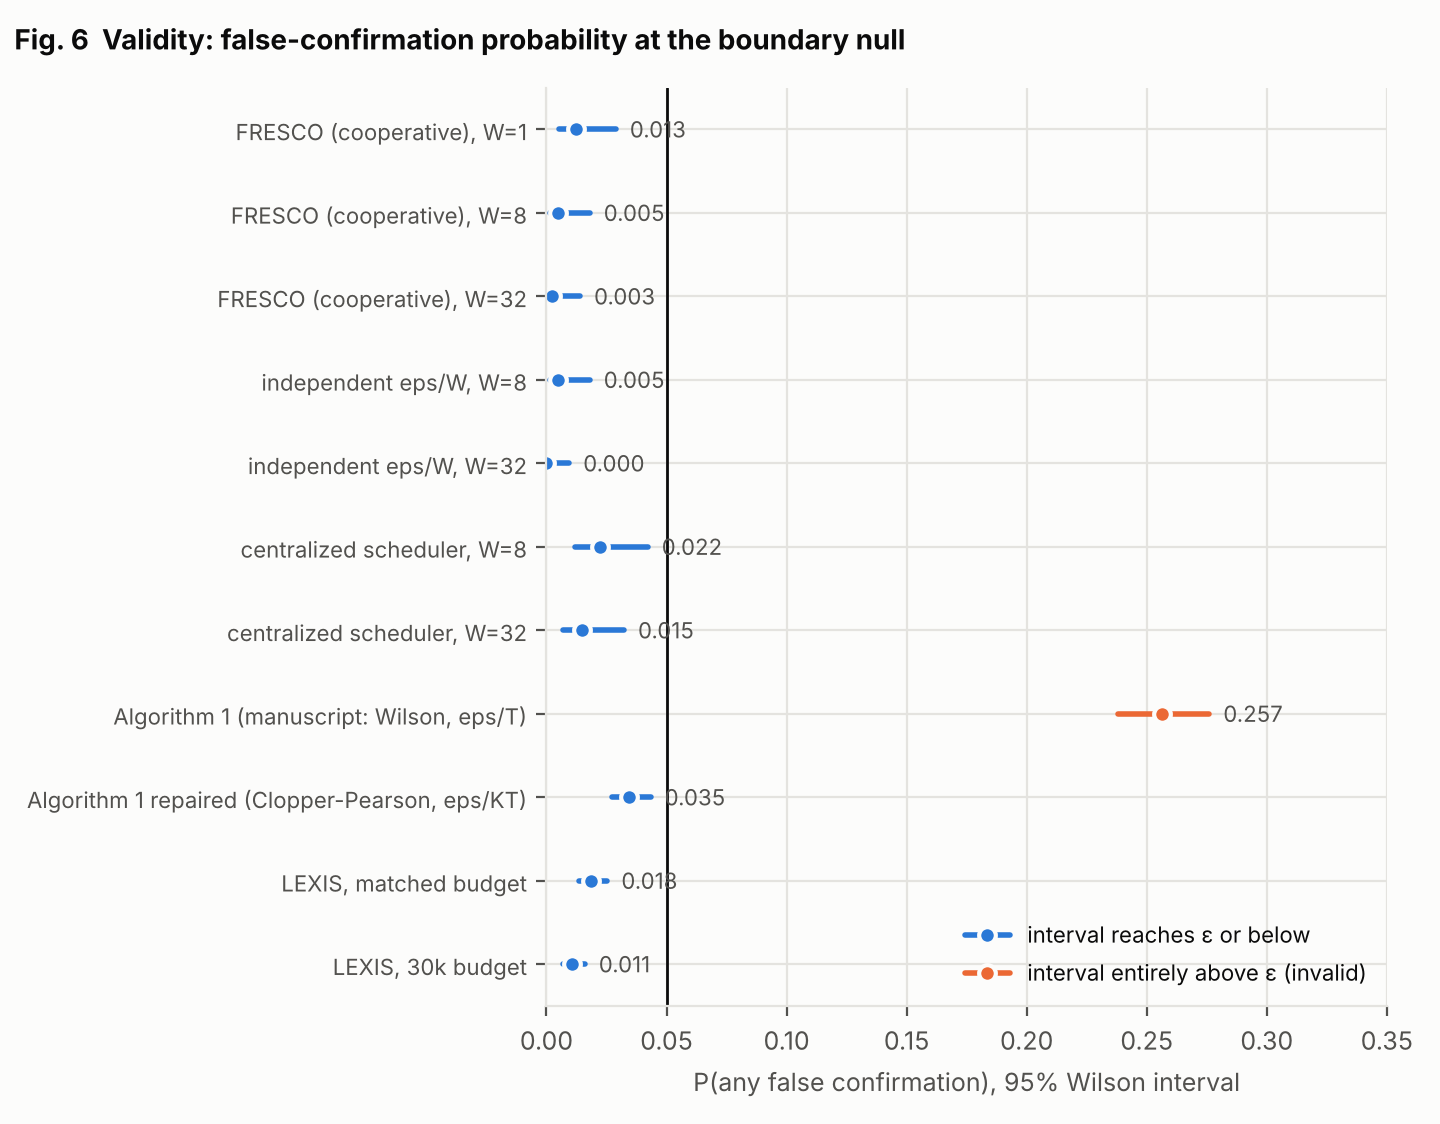
\includegraphics[width=0.82\linewidth]{fig6_validity.png}
\caption{Validity of all methods at the boundary null. Only Algorithm~1 as specified is invalid.}\label{fig:validity}
\end{figure}

\subsection{Scalability (RQ2)}
FRESCO's restricted mean time to the true margin fell from 27,955\,s at $W=1$ to 1,101\,s at $W=32$ on S1 (speedup 25.4$\times$, efficiency 0.79; Fig.~\ref{fig:scaling}); on S2 the speedup was at least 21.4$\times$ (38\% of single-worker runs were censored). Oracle calls to the margin stayed nearly flat (5.2k at $W=1$, 6.6k at $W=32$, overlapping CIs), messages per oracle call grew from 3.34 to 3.71, and the ledger processed about 10 operations per virtual second at $W=32$. Weak-scaling efficiency was 0.81--0.97 up to $W=16$ and 0.71 [0.53, 0.96] at $W=32$. After a 60\,s ledger crash, a 120\,s crash of half the workers, or a 300\,s partition of half the workers, throughput returned to 90\% of its pre-fault level within one 20\,s measurement bucket; lost work matched the arithmetic loss (Fig.~\ref{fig:recovery}).

\begin{figure}[t]\centering
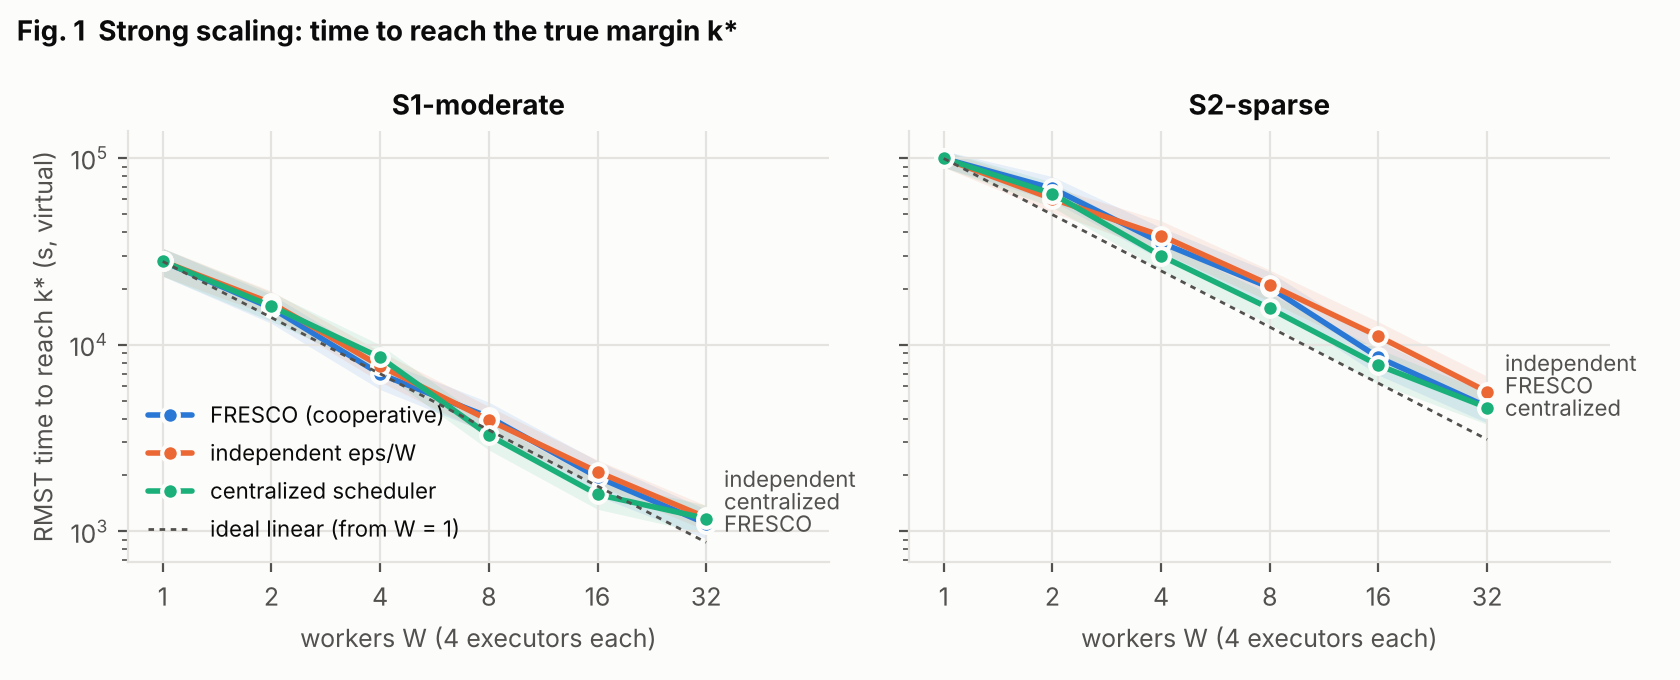
\includegraphics[width=\linewidth]{fig1_strong_scaling.png}\\[2mm]
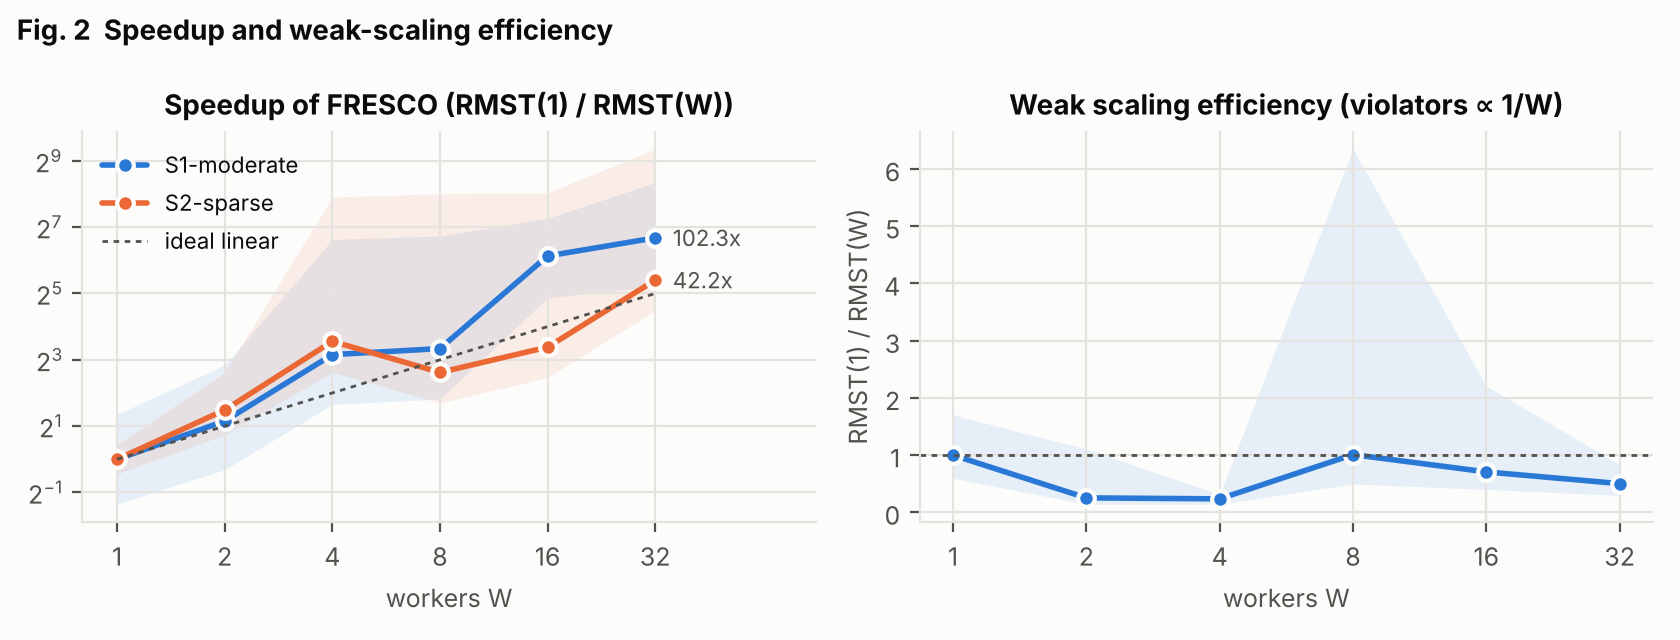
\includegraphics[width=\linewidth]{fig2_speedup_weak.png}
\caption{Strong scaling of time to the true margin for three methods (top; shaded: 95\% bootstrap CI) and FRESCO speedup and weak-scaling efficiency (bottom).}\label{fig:scaling}
\end{figure}

\begin{figure}[t]\centering
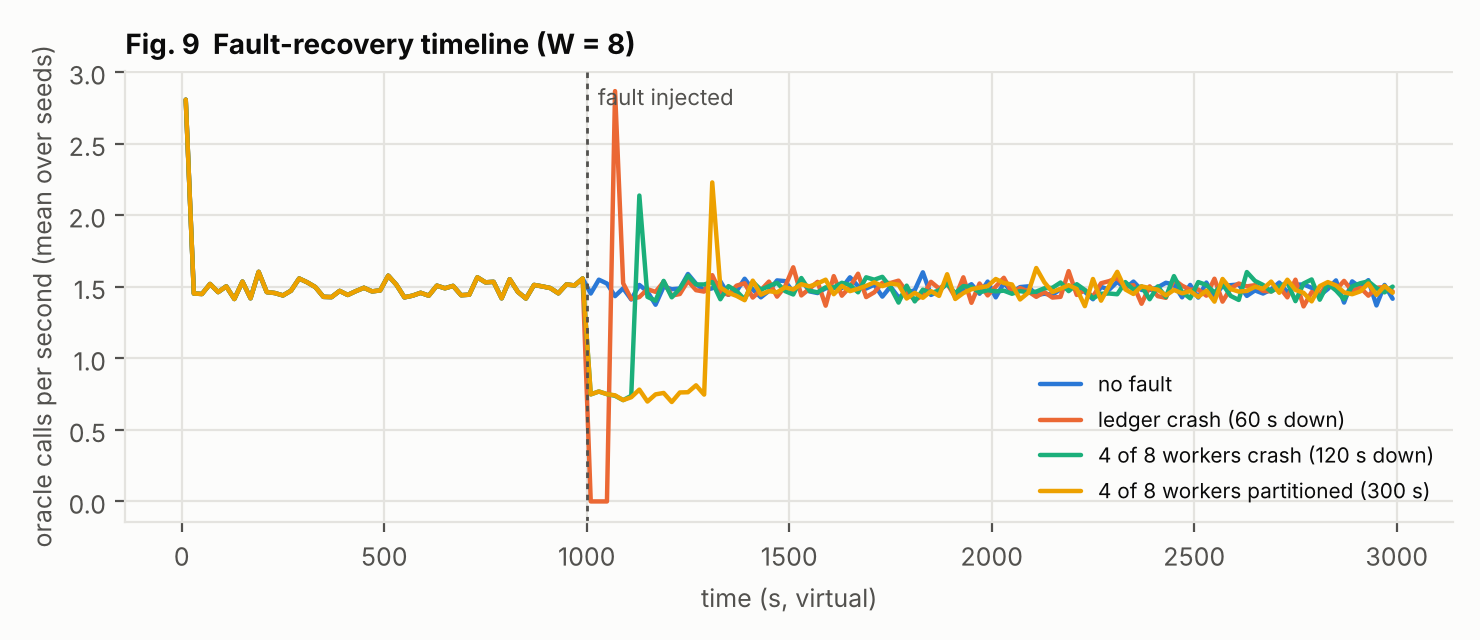
\includegraphics[width=0.85\linewidth]{fig9_recovery.png}
\caption{Oracle-call throughput around injected faults ($W=8$, mean of 30 seeds).}\label{fig:recovery}
\end{figure}

\subsection{Does cooperation help? (RQ3)}
No. In all 20 Holm-corrected comparisons (two scenarios, $W\in\{2,4,8,16,32\}$, against B1 and B3) we detected no difference: RMST ratios ranged from 0.77 to 1.14 against independent runs and 0.81 to 1.30 against the centralized scheduler, every 95\% CI contained 1, and every adjusted $p\ge0.94$ (Fig.~\ref{fig:km}). This agrees with the analysis that cooperation has no built-in statistical advantage---a shared budget spends over more registrations, roughly cancelling the union-bound saving---while frontier pruning saves only work at levels above the current margin. Effects smaller than a ratio of about 0.65 could not be detected.

\begin{figure}[t]\centering
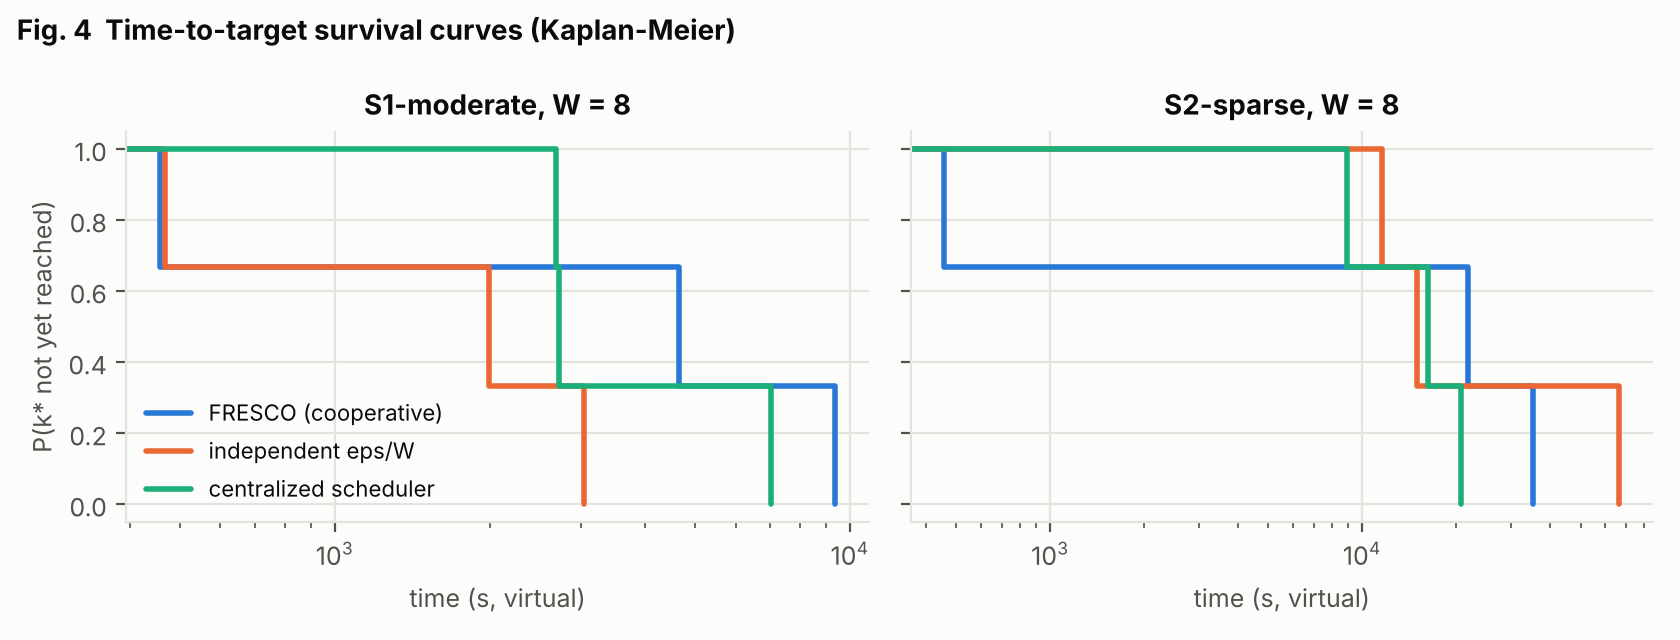
\includegraphics[width=\linewidth]{fig4_km_w8.png}
\caption{Kaplan--Meier curves of time to the true margin at $W=8$. Curves overlap in both scenarios.}\label{fig:km}
\end{figure}

\subsection{Sample efficiency and certificates (RQ4)}
At a matched budget of 1,160 oracle calls, repaired Algorithm~1 reached the true margin in 0.800 [0.782, 0.817] of S1 runs versus 0.246 [0.228, 0.266] for LEXIS, and 0.272 versus 0.043 on S2; LEXIS needed roughly 3--12$\times$ more calls (Table~\ref{tab:eff}). A post-hoc, explicitly exploratory reduction of the per-candidate cap did not close the gap. The cause is structural: Algorithm~1 screens each candidate with five trials and confirms only the top three, whereas LEXIS runs every opened null candidate to its cap and spreads effort over empty levels. Certificates covered in every run (coverage 1.000 [0.981, 1.000], both audit rules) but were loose: median $\bar\eta_k$ of 0.73--0.75 with $(r,t)=(3,1)$ and 0.39--0.40 with the gap rule $(10,4,\alpha_c=0.3)$, against true masses of 0--0.01. Ablations (Fig.~\ref{fig:abl}) confirmed the lease-policy fix (the earlier fixed-fraction policy was 1.7$\times$ slower at $W=32$), showed that cheap-first level weights cost 2.1$\times$ when cheap levels are barren, and that conservative crash imputation costs 1.7$\times$ under 20\% crashes, mostly recovered by replay mode.

\paragraph{Screening hybrid (preregistered follow-up).} LEXIS-S screens 40 candidates per level with five scouting trials on keys independent of confirmation keys, promotes the top three with error weights and bet priors fixed from the scouting data, and confirms each with an e-process capped at 30 trials; Theorem~\ref{thm:lexis} applies unchanged because weights and priors are registration information. Over 60,000 runs (Table~\ref{tab:hybrid}) it raised the probability of reaching $k^*$ at a matched budget from 0.246 to 0.756 on S1 and from 0.043 to 0.251 on S2, but stayed 2--5 points below repaired Algorithm~1; the preregistered non-inferiority margin of 0.05 was met in only 2 of 6 sensitivity comparisons, total oracle calls were unchanged (ratio $\approx1.00$, since screening dominates cost), and scouting-weighted spending gave no detectable benefit. LEXIS-S was markedly more conservative (false-confirmation rate 0.004 versus 0.034): a capped anytime-valid test does not use its full error budget at a fixed sample size, and that unused budget is the power it gives up.

\begin{table}[t]\centering\small
\caption{Screening hybrid vs repaired Algorithm~1 ($q=40$, $r_d=5$, $T=3$, cap $=30$; 2,000 runs per cell; 95\% Wilson intervals).}\label{tab:hybrid}
\begin{tabular}{lccc}
\toprule
Method & $\Prob$(reach $k^*$), S1 & $\Prob$(reach $k^*$), S2 & $\Prob$(false), boundary null \\\midrule
LEXIS (matched budget) & 0.246 & 0.043 & 0.018 \\
LEXIS-S (single pass) & 0.756 [0.737, 0.775] & 0.251 [0.232, 0.270] & 0.004 [0.002, 0.008] \\
Repaired Algorithm 1 (single pass) & 0.808 [0.790, 0.825] & 0.269 [0.250, 0.289] & 0.034 [0.027, 0.043] \\
LEXIS-S, multi-pass (5,000 calls) & 0.998 & 0.733 [0.713, 0.751] & 0.014 \\
Repaired Algorithm 1, multi-pass & 1.000 & 0.765 [0.746, 0.783] & 0.015 \\
\bottomrule\end{tabular}
\end{table}

\begin{table}[t]\centering\small
\caption{Probability of reaching the true margin $k^*=3$ (slot-level, single process; 2,000 runs each).}\label{tab:eff}
\begin{tabular}{llcc}
\toprule
Instance & Method & $\Prob$(reach $k^*$) & Median calls when reached \\\midrule
S1 & Algorithm 1 repaired ($\le$1,160 calls) & 0.800 [0.782, 0.817] & 810 \\
S1 & LEXIS, matched 1,160 calls & 0.246 [0.228, 0.266] & 552 \\
S1 & LEXIS, 30,000 calls & 0.998 [0.994, 0.999] & 2,993 \\
S2 & Algorithm 1 repaired & 0.272 [0.252, 0.291] & 810 \\
S2 & LEXIS, matched & 0.043 [0.035, 0.053] & 544 \\
S2 & LEXIS, 30,000 calls & 0.782 [0.764, 0.800] & 10,011 \\
\bottomrule\end{tabular}
\end{table}

\begin{figure}[t]\centering
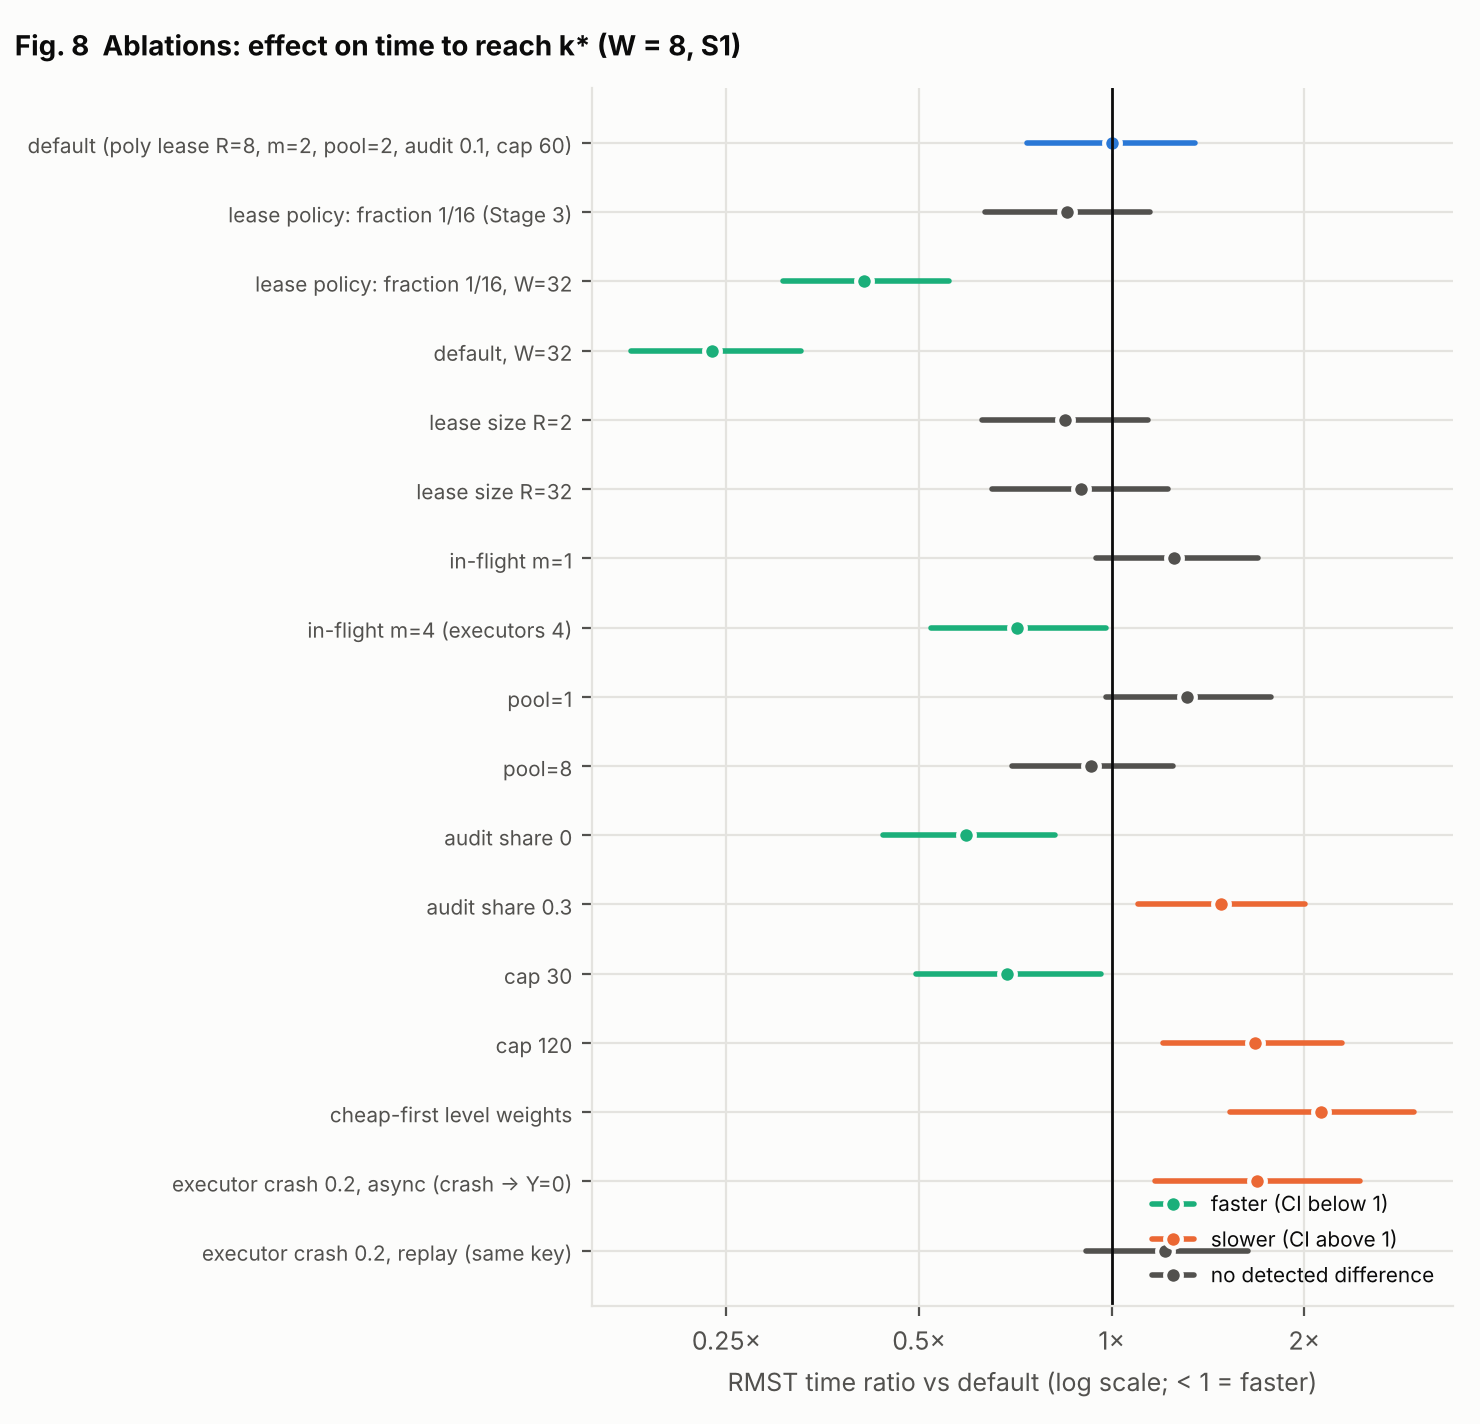
\includegraphics[width=0.82\linewidth]{fig8_ablations.png}
\caption{Component ablations at $W=8$ on S1 (RMST ratio relative to the default; 95\% CI).}\label{fig:abl}
\end{figure}

\begin{table}[t]\centering\small
\caption{Preregistered hypotheses and verdicts (synthetic evidence).}\label{tab:verdicts}
\begin{tabularx}{\linewidth}{lX>{\raggedright\arraybackslash}p{4.4cm}}
\toprule
Hypothesis & Criterion & Verdict \\\midrule
H-valid-sim & Wilson lower bound $\le\varepsilon$ in all FRESCO configurations & supported \\
H-rules & removed rule gives lower bound $>\varepsilon$ & supported for 3 of 4 rules \\
H-alg1 & specified Algorithm 1 exceeds $\varepsilon$, repaired does not & supported \\
H-vs-Alg1 & LEXIS reaches $k^*$ at least as often at matched budget & \textbf{refuted} \\
H6-noninf & LEXIS-S within 0.05 of repaired Algorithm 1 & not supported (2/6 settings) \\
H-speed & speedup CI lower bound $\ge16$ at $W=32$ & supported (25.4$\times$) \\
H-coop & cooperative FRESCO faster than B1 and B3 & \textbf{not supported} \\
H-overhead & $\le10$ messages per call, $\le100$ ledger ops/s & supported \\
H-recover & 90\% throughput within $2\times$ outage & supported \\
H-cert & coverage $\ge0.95$ & supported; certificates loose \\
H-valid-real & measured fault profiles imply inflation & \todo{TO RUN} \\
\bottomrule\end{tabularx}
\end{table}

\subsection{Real-agent experiments}\label{sec:realprotocol}
These have \emph{not} been run; Table~\ref{tab:real} lists the required evidence. The protocol: (1) profile 2,000 episodes per open-weight model to estimate timeout and crash rates separately for violating and benign trajectories and measure redelivery rates of common queue configurations, then rerun the fault-injection study with the measured rates; (2) replay 200 completed slots to verify seeded determinism; (3) compare FRESCO with B0b, B1 and B3 on 20 MARGIN-Bench scenario families with cluster bootstrap over families; (4) report authorized-task completion on paired counterparts; (5) re-confirm witnesses across models with fresh keys.

\begin{table}[t]\centering\small
\caption{Real-agent result shells. No value may be filled except from executed runs.}\label{tab:real}
\begin{tabular}{lll}
\toprule
Quantity & Model A & Model B \\\midrule
Timeout/crash rate by outcome $(c_0,c_1)$ & \todo{TO RUN} & \todo{TO RUN} \\
Replay determinism (\% trace-hash match) & \todo{TO RUN} & \todo{TO RUN} \\
Implied false-confirmation inflation per removed rule & \todo{TO RUN} & \todo{TO RUN} \\
RMST time to $\bhat$: FRESCO / B1 / B3 & \todo{TO RUN} & \todo{TO RUN} \\
Per-surface $\bhat$ and censoring fraction & \todo{TO RUN} & \todo{TO RUN} \\
Authorized-task completion & \todo{TO RUN} & \todo{TO RUN} \\
Cross-model witness transfer rate & \todo{TO RUN} & \todo{TO RUN} \\
\bottomrule\end{tabular}
\end{table}

% -----------------------------------------------------------------------------
\section{Discussion and failure analysis}\label{sec:discussion}

\paragraph{What the evidence supports.} The defensible contribution is \emph{fault-tolerant validity}: an evaluation harness can be parallelised to tens of workers with near-linear speedup and negligible coordination while its reported margins keep their stated error level under faults that, with ordinary engineering defaults, inflate that error several-fold. The rules are cheap---one ledger write per episode and a write-once constraint---and they remove failure modes whose error is unbounded in the limit.

\paragraph{What it does not support.} Cooperation did not help, and sequential confirmation did not improve sample efficiency. The screening hybrid showed that LEXIS's deficit came from search structure rather than from its statistics, yet even with screening the anytime-valid confirmation remained 2--5 points less powerful than an exact fixed-$n$ test, and early stopping saved no calls because screening dominates cost. What the e-process buys is continuation, validity under arbitrary stopping, and a natural fit to asynchronous evidence streams---not efficiency. Since the FRESCO rules other than in-order commit apply equally to fixed-$n$ confirmations, the most practical recommendation is repaired Algorithm~1 (or LEXIS-S where anytime properties matter) executed under those rules. The certificates are honest but coarse; informative statements at the 1--5\% level need thousands of audits per level or a certified gap above $\alpha$.

\paragraph{When FRESCO fails.} Validity is lost if episodes share hidden state (e.g.\ memory not reset between slots), if the oracle has false positives (the guarantee then concerns the observed rate), or if keys leak to the generator. Efficiency collapses if violating episodes time out more often than benign ones, since conservative imputation then hides them; replay mode or longer deadlines are required, and deadlines must be preregistered as statistical parameters.

\paragraph{Implications for MARGIN-Bench.} Its Algorithm~1 should either adopt the exact $\varepsilon/(KT)$ repair, which costs no efficiency in our experiments, or the screening-plus-e-process hybrid; and any distributed harness used for it should implement at least deduplication, in-order consumption and the fresh-retry ban.

% -----------------------------------------------------------------------------
\section{Threats to validity}\label{sec:threats}
\textit{Construct:} synthetic oracles and latency/crash models are assumptions; effect sizes of rule violations in real harnesses may be smaller or larger. \textit{Internal:} default parameters (cap, audit share, lease size) were not tuned and are not time-optimal; one post-hoc variant is labelled exploratory. \textit{Statistical:} 100 seeds per cell bound detectable effects; censoring at a common horizon is handled by RMST; seeds share random streams across methods by design. \textit{External:} the simulated generator is non-adaptive; adaptive attackers add sequential depth that may limit scaling. \textit{Implementation:} the production database ledger is specified but not executed; coordination cost is measured in virtual time.

\section{Limitations and negative results}\label{sec:limits}
(i) No real-agent results. (ii) No cooperative speed-up was detected. (iii) LEXIS, even with screening (LEXIS-S), is somewhat less powerful than a repaired fixed design at matched budgets. (iv) Certificates are loose at realistic audit budgets. (v) The global-budget rule's necessity was not established at $W=8$ in the system-level study, although it follows analytically for larger $W$. (vi) Byzantine executors are not covered; verifiable confirmation checks computation, not outcomes. (vii) Bit-reproducible epoch mode, an ASHA-style scheduler baseline and the database adapter are not yet implemented.

\section{Reproducibility and data availability}\label{sec:repro}
All code, configurations, raw results (JSON lines with configuration hashes and code revisions), analysis scripts and figures are in the project repository \todo{INSERT PERMANENT ARCHIVE DOI}. \texttt{experiments/run\_all.sh} regenerates every number and figure in about two hours on four cores; \texttt{python -m pytest tests} runs 42 unit, property-based and integration tests; the simulator is deterministic given configuration and seed. For real-agent runs, the run key is committed by hash before execution and revealed afterwards, so every slot key can be recomputed and checked against stored traces.

\section{Future work}\label{sec:future}
Execute the real-agent protocol; close the residual power gap of the screening hybrid (mixture bets, adaptive allocation of confirmation trials), each under its own preregistration; adaptive level scheduling that beats the factor-$K$ price on structured instances; tighter certificates via adaptive audit allocation; Byzantine-tolerant executors with attestation for third-party compute; and extension of the evaluation to authorization-race scenarios in multi-agent delegation.

\section{Conclusion}\label{sec:conclusion}
Statistical guarantees of LLM-agent security evaluation depend on how episodes are executed. We proved that six simple protocol rules make sequential margin confirmation valid independently of scheduling and faults, showed that each common executor default can break it, and demonstrated in simulation near-linear scaling at negligible coordination cost. Two hypotheses we expected to hold did not: cooperation brought no speed-up, and our sequential procedure was less sample-efficient than a repaired fixed design---a screening hybrid narrowed but did not close that gap---while the comparison exposed an error in the original benchmark's estimator. Real-agent validation remains to be done.

% -----------------------------------------------------------------------------
\section*{Declarations}
\noindent\textbf{Funding.} \todo{INSERT TRUE FUNDING INFORMATION OR ``No funding was received''.}\\
\textbf{Competing interests.} \todo{AUTHORS TO DISCLOSE.}\\
\textbf{Ethics approval.} Not applicable to the simulation study; the real-agent protocol uses sandboxed mock tools and no human participants \todo{CONFIRM BEFORE REAL-AGENT RUNS}.\\
\textbf{Data availability.} Synthetic results are released with the code \todo{ARCHIVE DOI}. No real-agent data exist yet.\\
\textbf{Code availability.} \todo{REPOSITORY URL AND ARCHIVE DOI}.\\
\textbf{Author contributions.} \todo{CRediT STATEMENT}.\\
\textbf{Use of generative AI.} \todo{AUTHORS MUST DISCLOSE: substantial parts of the design, code, analysis and text of this working manuscript were drafted with an AI assistant and must be verified and declared according to the journal's policy.}

\bibliographystyle{unsrtnat}
\bibliography{references}
\end{document}
